\section{Resultados}

\subsection{Resultados del proyecto}

A continuación se van a mostrar algunos ejemplos de las predicciones obtenidas con los modelos que mejores resultados han obtenido, que son los que han sido entrenados con el juego de datos de entrenamiento \textit{filtro 100x40}.

\begin{figure}[H]
	\centering
	\begin{subfigure}[h]{0.45\linewidth}
		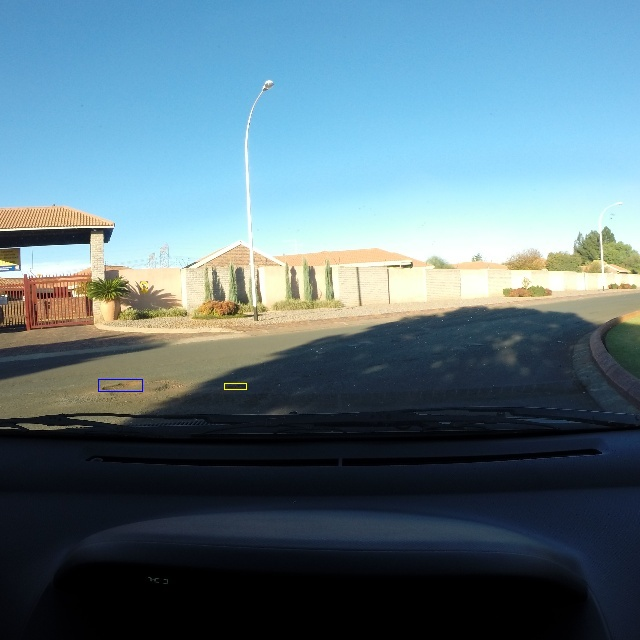
\includegraphics[width=\linewidth]{images/results_a_gt.jpg}
		\caption{Socavones a detectar}
	\end{subfigure}
	\begin{subfigure}[h]{0.45\linewidth}
		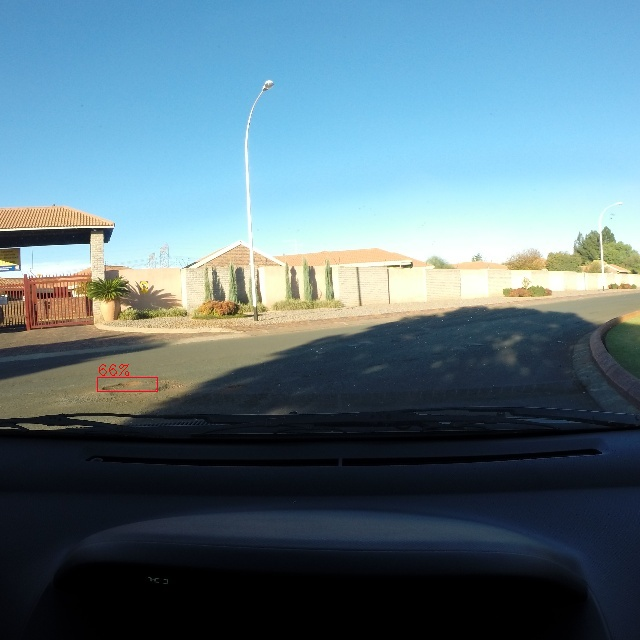
\includegraphics[width=\linewidth]{images/results_a_yolo_v3_256.jpg}
		\caption{YOLO v3 tamaño 256x256}
	\end{subfigure}
	\begin{subfigure}[h]{0.45\linewidth}
		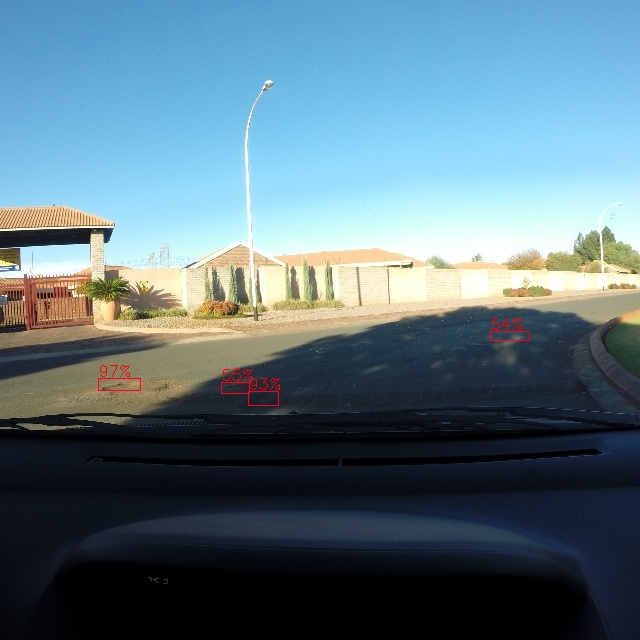
\includegraphics[width=\linewidth]{images/results_a_yolo_v3_416.jpg}
		\caption{YOLO v3 tamaño 416x416}
	\end{subfigure}
	\begin{subfigure}[h]{0.45\linewidth}
		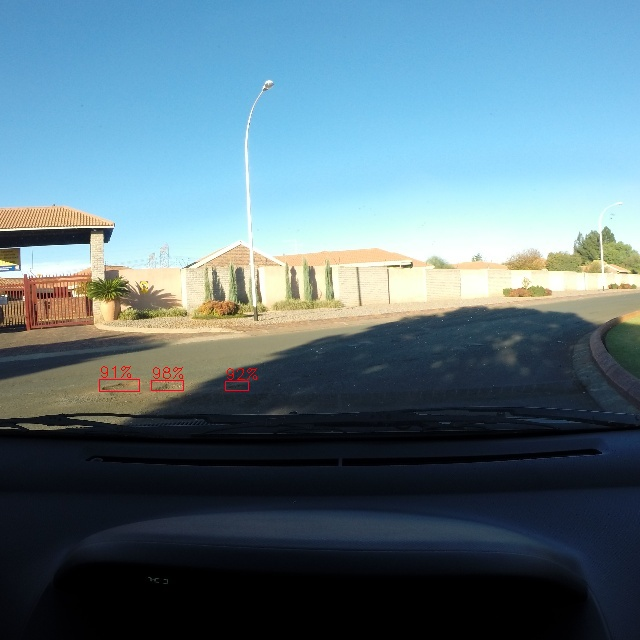
\includegraphics[width=\linewidth]{images/results_a_yolo_v3_640.jpg}
		\caption{YOLO v3 tamaño 640x640}
	\end{subfigure}
	\caption{Ejemplo de predicción con modelos YOLO v3 de distintos tamaños. Arriba a la izquierda, la imagen con los socavones a detectar en azul y en amarillo los socavones que fueron descartados por el filtro 100x40. En el resto de las imágenes se pueden ver las predicciones realizadas en rojo.}
	\label{fig:resultsav3}
\end{figure}

En la figura \ref{fig:resultsav3} se muestran las predicciones realizadas por los modelos \textit{YOLO v3}. Se trata de una imagen en la que originalmente se han etiquetado 2 socavones, uno de los cuales se ha descartado por ser demasiado pequeño. También se puede observar que existe un defecto en el etiquetado, ya que entre los dos socavones etiquetados existe un tercer socavón sin etiquetar. Aún habiendo filtrado los socavones pequeños se puede comprobar que el modelo es capaz de detectarlos (en los modelos de tamaño 416x416 y 640x640). También se puede observar que el modelo de tamaño 640x640 es capaz de detectar el socavón sin etiquetar.

En la figura \ref{fig:resultsav3tiny} se muestran las predicciones realizadas por los modelos \textit{YOLO v3 tiny} para la misma imagen. Únicamente el modelo de tamaño 416x416 es capaz de detectar el socavón, aunque lo hace de manera poco precisa ya que la región detectada es demasiado grande y abarca también al socavón sin etiquetar.

\begin{figure}[H]
	\centering
	\begin{subfigure}[h]{0.45\linewidth}
		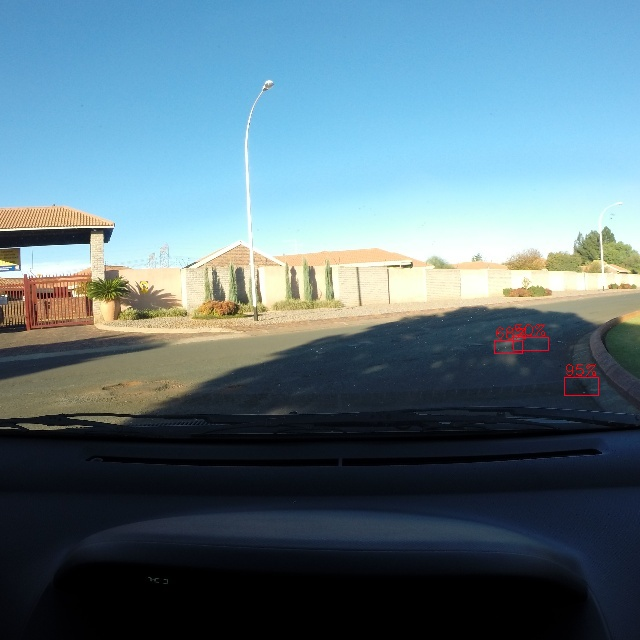
\includegraphics[width=\linewidth]{images/results_a_yolo_v3_tiny_256.jpg}
		\caption{YOLO v3 tiny tamaño 256x256}
	\end{subfigure}
	\begin{subfigure}[h]{0.45\linewidth}
		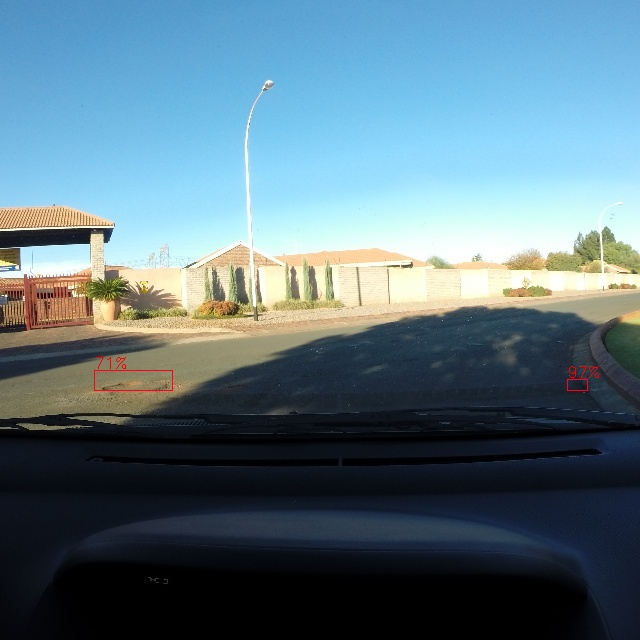
\includegraphics[width=\linewidth]{images/results_a_yolo_v3_tiny_416.jpg}
		\caption{YOLO v3 tiny tamaño 416x416}
	\end{subfigure}
	\caption{Misma predicción que en la figura \ref{fig:resultsav3}, pero en esta ocasión con modelos YOLO v3 tiny.}
	\label{fig:resultsav3tiny}
\end{figure}

\begin{figure}[H]
	\centering
	\begin{subfigure}[h]{0.45\linewidth}
		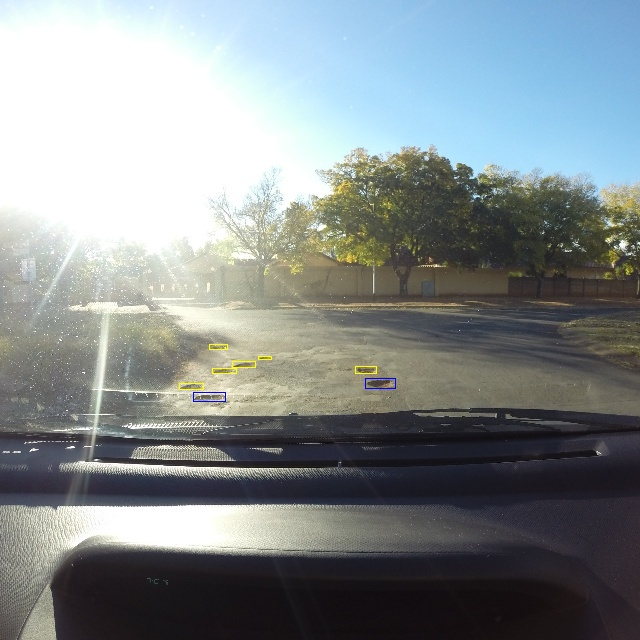
\includegraphics[width=\linewidth]{images/results_b_gt.jpg}
		\caption{Socavones a detectar}
	\end{subfigure}
	\begin{subfigure}[h]{0.45\linewidth}
		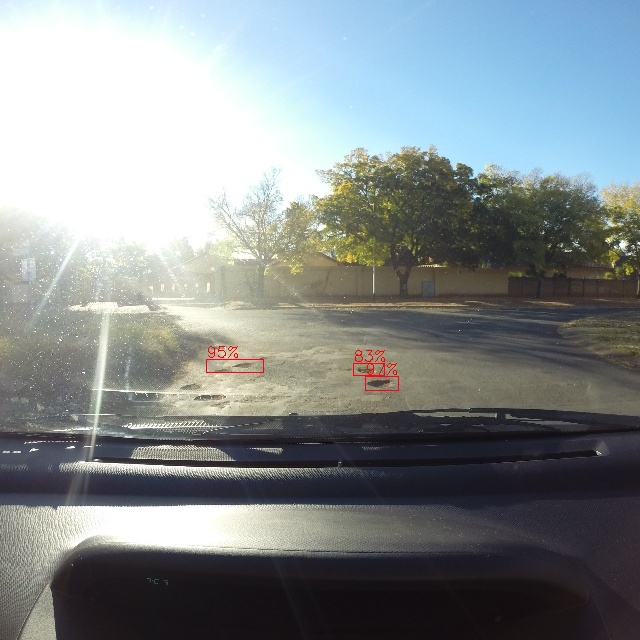
\includegraphics[width=\linewidth]{images/results_b_yolo_v3_256.jpg}
		\caption{YOLO v3 tamaño 256x256}
	\end{subfigure}
	\begin{subfigure}[h]{0.45\linewidth}
		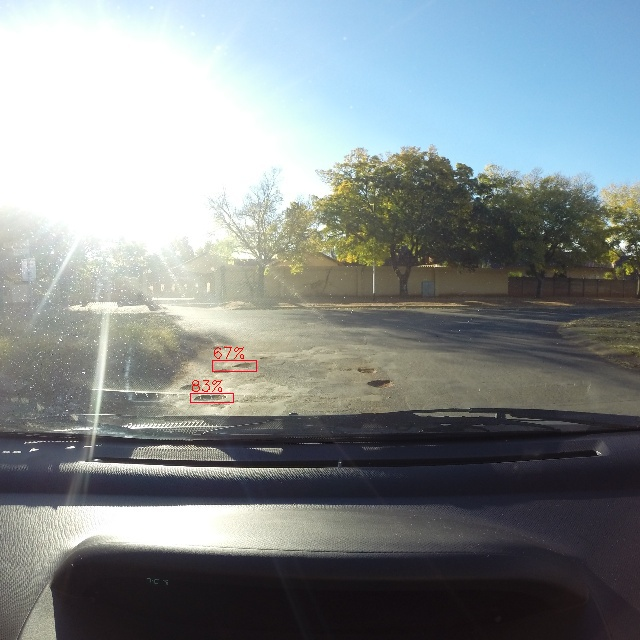
\includegraphics[width=\linewidth]{images/results_b_yolo_v3_416.jpg}
		\caption{YOLO v3 tamaño 416x416}
	\end{subfigure}
	\begin{subfigure}[h]{0.45\linewidth}
		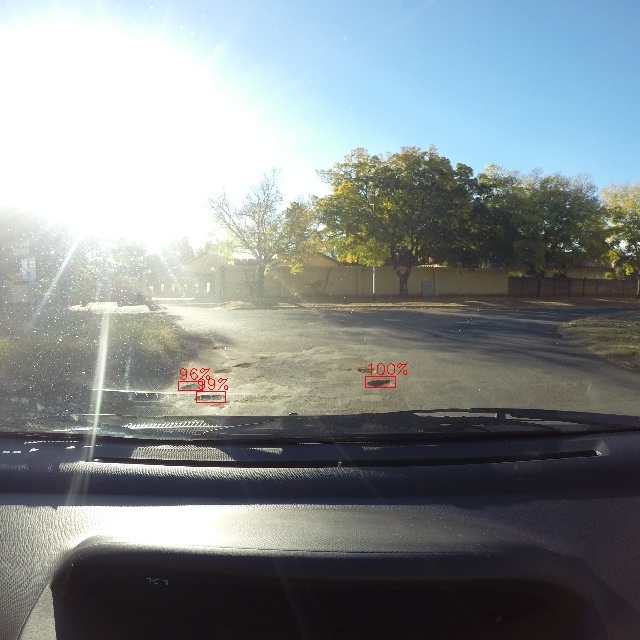
\includegraphics[width=\linewidth]{images/results_b_yolo_v3_640.jpg}
		\caption{YOLO v3 tamaño 640x640}
	\end{subfigure}
	\caption{Ejemplo de predicción con modelos YOLO v3 de distintos tamaños. Arriba a la izquierda, la imagen con los socavones a detectar en azul y en amarillo los socavones que fueron descartados por el filtro 100x40. En el resto de las imágenes se pueden ver las predicciones realizadas en rojo.}
	\label{fig:resultsbv3}
\end{figure}

\begin{figure}[H]
	\centering
	\begin{subfigure}[h]{0.45\linewidth}
		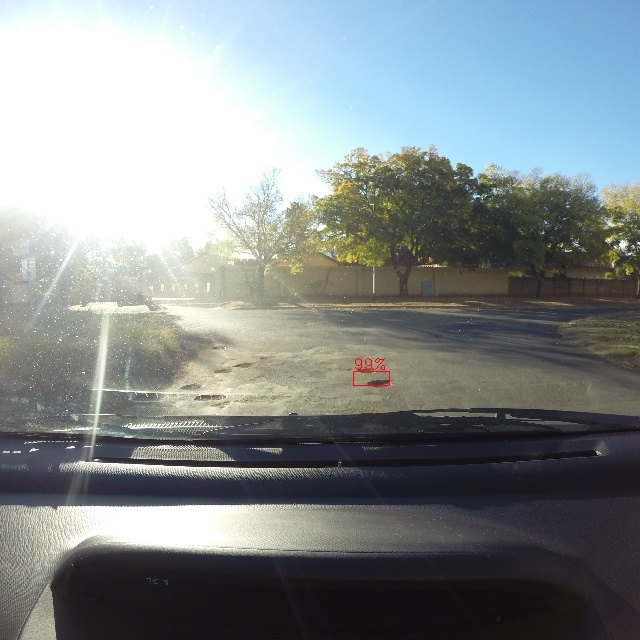
\includegraphics[width=\linewidth]{images/results_b_yolo_v3_tiny_256.jpg}
		\caption{YOLO v3 tiny tamaño 256x256}
	\end{subfigure}
	\begin{subfigure}[h]{0.45\linewidth}
		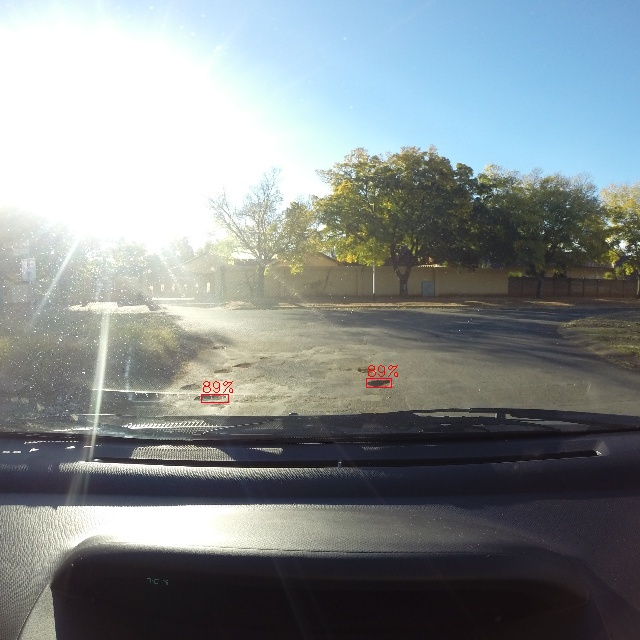
\includegraphics[width=\linewidth]{images/results_b_yolo_v3_tiny_416.jpg}
		\caption{YOLO v3 tiny tamaño 416x416}
	\end{subfigure}
	\caption{Misma predicción que en la figura \ref{fig:resultsbv3}, pero en esta ocasión con modelos YOLO v3 tiny.}
	\label{fig:resultsbv3tiny}
\end{figure}

{\color{red} \textbf{!!! TODO}}